\documentclass{beamer}

\usepackage[utf8]{inputenc}
\usepackage[english]{babel}

\usepackage{amsmath}
\usepackage{nicefrac}

\usepackage{minted}
\usepackage{fontspec}

\usepackage{xcolor}
\usepackage{graphicx}

\usemintedstyle{friendly}
\setmonofont{Source Code Pro}
\usetheme{metropolis}

\newcommand{\then}{\Rightarrow}

\title{Relaciones entre conjuntos}
\author{Matemática estructural y lógica}
\institute{ISIS-1104}
\date{}

\begin{document}

\frame{\titlepage}

\begin{frame}[fragile]
    \frametitle{¿Qué es una relación?}
    \begin{itemize}
        \item Si $A$ y $B$ son conjuntos, definimos el conjunto de relaciones entre $A$ y $B$ como:
    $$A \leftrightarrow B = \mathcal{P}(A \times B)$$
\item Es decir, todo elemento de $A \leftrightarrow B$ es un subconjunto de $A \times B$.
\item Decimos que $R$ es una relación entre $A$ y $B$ si $R \in A \leftrightarrow B$.
    \end{itemize}
\end{frame}

\begin{frame}[fragile]
    \frametitle{¿Qué es una relación?}
    \begin{itemize}
        \item Si $R \in A \leftrightarrow B$, sabemos que $R$ debe estar conformado por algunos elementos de $A \times B$. 
        \item Es decir, $R$ es un conjunto de parejas ordenadas de $A$ y $B$.
        \item En ese orden de ideas, introducimos la siguiente notación
            $$aRb \equiv (a, b) \in R$$
        \item Usualmente $aRb$ se lee "$a$ está relacionado con $b$ por $R$".
    \end{itemize}
\end{frame}

\begin{frame}[fragile]
    \frametitle{Un par de ejemplos}
    Sea $R \in \mathbb{Z} \leftrightarrow \mathbb{Z} $ la relación definida por el siguiente enunciado:
    $$aRb \equiv \text{"$a$" es igual a el valor absoluto de "$b$"}$$
    \begin{center}
        ¿Qué elementos de $ \mathbb{Z}$ están relacionados por $R$?
    \end{center}
    Sea $S \in \mathbb{Z} \leftrightarrow \mathbb{Z} $ la relación definida por el siguiente enunciado:
    $$aSb \equiv \text{ $a - b$ es par }$$
    \begin{center}
        ¿Qué elementos de $\mathbb{Z}$ están relacionados por $R$?
    \end{center}
\end{frame}

\begin{frame}[fragile]
    \frametitle{Algunas definiciones}
    Si $R \in A \leftrightarrow B$:
    \begin{itemize}
        \item $A$ es el dominio de $R$.
        \item $B$ es el codominio de $R$.
        \item $\text{dom}(R) = \{a : A \mid (\exists b: B \mid : aRb)\}$ es el dominio de definición de $R$
        \item $\text{ran}(R) = \{b : B \mid (\exists a: A \mid : aRb)\}$ es el rango de $R$
        \item $R^T = \{(b, a) : (B \times A) \mid aRb\}$ es la inversa (o transpuesta) de $R$
    \end{itemize}
    \begin{center}
        ¿Cuáles son los dominios, codomonios, dominios de definición, rangos e inversas de nuestros ejemplos?
    \end{center}
\end{frame}

\begin{frame}[fragile]
    \frametitle{Tipos de relaciones: Total}
    Decimos que $R \in A \leftrightarrow B$ es total si
    $$(\forall a:A \mid : (\exists b:B \mid : aRb))$$
    Equivalentemente, podemos decir que $R$ es total si 
    $$\text{dom}(R) = A$$
    \begin{center}
        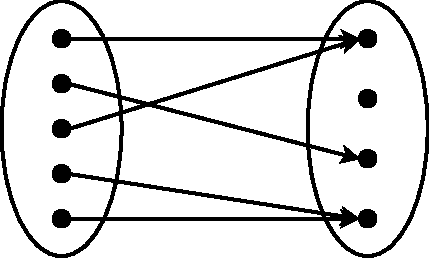
\includegraphics[width=0.5\linewidth]{images/total.pdf}
    \end{center}
\end{frame}

\begin{frame}[fragile]
    \frametitle{Tipos de relaciones: Sobreyectiva}
    Decimos que $R \in A \leftrightarrow B$ es sobreyectiva si
    $$(\forall b:B \mid : (\exists a:A \mid : aRb))$$
    Equivalentemente, podemos decir que $R$ es sobreyectiva si 
    $$\text{ran}(R) = B$$
    \begin{center}
        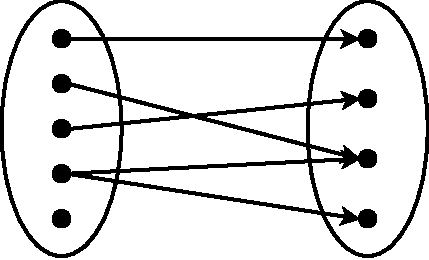
\includegraphics[width=0.5\linewidth]{images/surjective.pdf}
    \end{center}
\end{frame}

\begin{frame}[fragile]
    \frametitle{Tipos de relaciones: Función}
    Decimos que $R \in A \leftrightarrow B$ es función si
    $$(\forall a:A \mid aRb_{1} \land aRb_{2}: b_1 = b_2)$$
    Equivalentemente, podemos decir que  
    \begin{center}
        $R$ es función $\equiv$ $R^T$ es inyectiva
    \end{center}
    \begin{center}
        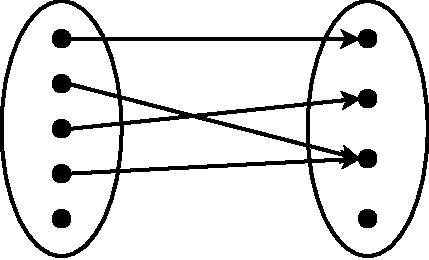
\includegraphics[width=0.5\linewidth]{images/function.pdf}
    \end{center}
\end{frame}

\begin{frame}[fragile]
    \frametitle{Tipos de relaciones: Inyectiva}
    Decimos que $R \in A \leftrightarrow B$ es inyectiva si
    $$(\forall b:B \mid a_{1}Rb \land a_{2}Rb: a_1 = a_2)$$
    Equivalentemente, podemos decir que  
    \begin{center}
        $R$ es inyectiva $\equiv$ $R^T$ es función
    \end{center}
    \begin{center}
        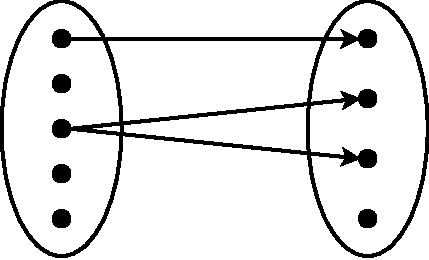
\includegraphics[width=0.5\linewidth]{images/injective.pdf}
    \end{center}
\end{frame}

\begin{frame}[fragile]
    \frametitle{Tipos de relaciones: Función total y Biyección}
    \begin{itemize}
        \item Decimos que $R \in A \leftrightarrow B$ es función total si es función y es total
        \item Decimos que $R \in A \leftrightarrow B$ es biyectiva si es función, inyectiva y sobreyectiva.
        \item $R$ es biyectiva $\equiv$ $R^T$ es biyectiva
    \end{itemize}
\end{frame}

\begin{frame}[fragile]
    \frametitle{Composición de relaciones: Definición}
    Si tenemos $R \in A \leftrightarrow B$ y $S \in B \leftrightarrow C$ podemos \textbf{componerlas} para obtener una nueva relación
    $$a (R \circ S) c \equiv (\exists b: B \mid : aRb \land bSc)$$
    \begin{center}
        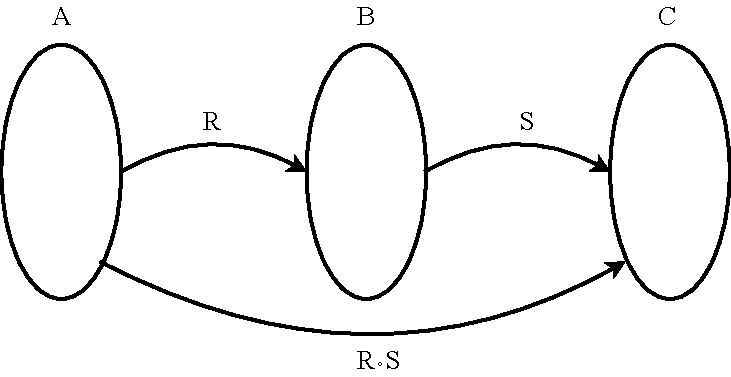
\includegraphics[width=0.7\linewidth]{images/composition.pdf}
    \end{center}
\end{frame}

\begin{frame}[fragile]
    \frametitle{Composición de relaciones: Asociatividad} 
    Si $R \in A \leftrightarrow B$, $S \in B \leftrightarrow C$ y $T \in C \leftrightarrow D$, entonces
    $$R \circ (S \circ T) = (R \circ S) \circ T$$
    \textbf{Demostración:} \\
    Queremos ver que si $a \in A$, $d \in D$
    $$a (R \circ (S \circ T)) d \equiv a ((R \circ S) \circ T) d$$
    Por definición de $\circ$
    $$a (R \circ (S \circ T)) d \equiv (\exists b: B \mid : a R b \land b (S \circ T) d)$$
    Por definición de $\circ$
    $$(\exists b: B \mid : a R b \land b (S \circ T) d) \equiv (\exists b: B \mid : a R b \land (\exists c: C \mid : bSc \land cTd))$$
\end{frame}

\begin{frame}[fragile]
    \frametitle{Composición de relaciones: Asociatividad} 
    Por anidamiento
    $$(\exists b \mid : a R b \land (\exists c \mid : bSc \land cTd)) \equiv (\exists b, c \mid : a R b \land bSc \land cTd)$$
    Por anidamiento
    $$(\exists b, c \mid : a R b \land bSc \land cTd) \equiv (\exists c \mid : (\exists b \mid : aRb \land bSc) \land cTd)$$
    Por definición de $\circ$
    $$(\exists c \mid : (\exists b \mid : aRb \land bSc) \land cTd) \equiv (\exists c \mid : a(R \circ S)c \land cTd)$$
    Por definición de $\circ$
    $$(\exists c \mid : a(R \circ S)c \land cTd) \equiv a((R \circ S) \circ T)d$$
\end{frame}

\begin{frame}[fragile]
    \frametitle{Composición de relaciones: Distribución} 
    Si $R \in A \leftrightarrow B$, $S \in B \leftrightarrow C$ y $T \in B \leftrightarrow C$, entonces
    $$ R \circ (S \cup T) = (R \circ S) \cup (R \circ T)$$
    \textbf{Demostración:} Para ustedes
    \vspace{165pt}
\end{frame}

\begin{frame}[fragile]
    \frametitle{Relaciones dentro de un mismo conjunto}
    Si $R \in A \leftrightarrow A$ decimos que:
    \begin{itemize}
        \item $R$ es reflexiva si $(\forall a:A \mid : aRa)$
        \item $R$ es irreflexiva si $(\forall a:A \mid : \lnot aRa)$
        \item $R$ es simétrica si $(\forall a, b:A \mid aRb : bRa)$
        \item $R$ es asimétrica si $(\forall a, b:A \mid aRb : \lnot bRa)$
        \item $R$ es antisimetrica si $(\forall a, b:A \mid aRb \land bRa : a = b)$
        \item $R$ es transitiva si $(\forall a, b, c:A \mid aRb \land bRc: aRc)$
    \end{itemize}
\end{frame}

\begin{frame}[fragile]
    \frametitle{Definiciones alternativas}
    Definimos la relación identidad $I \in A \leftrightarrow A$ como
    $$I = \{(a, a) \mid a \in A\}$$
    Si $R \in A \leftrightarrow A$ decimos que:
    \begin{itemize}
        \item $R$ es reflexiva si $I \subseteq R$
        \item $R$ es irreflexiva si $I \cap R = \varnothing$
        \item $R$ es simétrica si $R = R^T$
        \item $R$ es asimetrica si $R \cap R^T = \varnothing$
        \item $R$ es antisimétrica si $R \cap R^T \subseteq I$
        \item $R$ es transitiva si $R \circ R \subset R$
    \end{itemize}
\end{frame}

\begin{frame}[fragile]
    \frametitle{Definiciones alternativas}
    Demostremos que
    $$(\forall a:A \mid : aRa) \equiv (I \subseteq R)$$
    \textbf{Demostración:} \\
    Por definición de $\subseteq$
    $$(I \subseteq R) \equiv (\forall a, b \mid : (a,b) \in I \then (a,b) \in R)$$
    Por notación de relación
    $$(\forall a, b \mid : (a,b) \in I \then a,b \in R) \equiv (\forall a, b \mid : aIb \then aRb)$$
    Por definición de identidad
    $$(\forall a, b \mid : aIb \then aRb) \equiv (\forall a, b \mid : (a=b) \then aRb )$$
\end{frame}

\begin{frame}[fragile]
    \frametitle{Definiciones alternativas}
    Por anidamiento
    $$(\forall a, b \mid : (a=b) \then aRb ) \equiv (\forall a \mid : (\forall b \mid : ((a = b) \then aRb)))$$
    Por trueque
    $$(\forall a \mid : (\forall b \mid : (a = b) \then aRb)) \equiv (\forall a \mid : (\forall b \mid (a =  b) : aRb))$$
    Por regla de un punto
    $$(\forall a \mid : (\forall b \mid (a =  b) : aRb)) \equiv (\forall A \mid : aRa)$$
\end{frame}

\begin{frame}[fragile]
    \frametitle{Definiciones alternativas}
    Ahora ustedes demuestren que
    $$(\forall a:A \mid : \lnot aRa) \equiv (I \cap R = \varnothing)$$
    \vspace{160pt}
\end{frame}

\begin{frame}[fragile]
    \frametitle{Relaciones de equivalencia: Definición}
    Sea $R \in A \leftrightarrow A$, decimos que $R$ es una \textbf{relación de equivalencia} si $R$ es reflexiva, simétrica y transitiva.\\
    \textbf{Ejemplos:}
    \begin{itemize}
        \item $R : LL104 \leftrightarrow LL104$ definida como
            $$aRb \equiv \text{los códigos de $a$ y $b$ terminan en el mismo número}$$
        \item $S: \mathbb{Z} \leftrightarrow \mathbb{Z}$ definida como 
            $$aSb \equiv (a - b)\text{ es multiplo de 3}$$ 
        \item $T: \mathbb{Z} \leftrightarrow \mathbb{Z}$ definida como
            $$aTb \equiv \text{$a$ y $b$ son primos}$$
    \end{itemize}
\end{frame}

\begin{frame}[fragile]
    \frametitle{Relaciones de equivalencia: Clases}
    Sea $R \in A \leftrightarrow A$ una relación de equivalencia y $a \in A$.
    Definimos la clase de equivalencia de $a$ como:
    $$[a]_{R} = \{b \in A \mid aRb\}$$
    En otras palabras, la clase de $a$ es el conjunto de todos los elementos que se relacionan con $a$.\\
    \begin{center}
        ¿Cuáles y cuántas son las clases de equivalencia de los ejemplos anteriores?
    \end{center}
\end{frame}

\begin{frame}[fragile]
    \frametitle{Relaciones de orden parcial: Definición}
    Sea $R \in A \leftrightarrow A$, decimos que $R$ es un \textbf{orden parcial} si es reflexiva, antisimétrica y transitiva.\\
    \textbf{Ejemplos:}
    \begin{itemize}
        \item $\leq: \mathbb{Z} \leftrightarrow \mathbb{Z}$  
        \item $\subseteq: \mathcal{U} \leftrightarrow \mathcal{U}$  
        \item $R : LL104 \leftrightarrow LL104$ definida como
            $$aRb \equiv \text{el último número del código de $a$ es $\leq$ que el de $b$}$$
    \end{itemize}
\end{frame}

\begin{frame}[fragile]
    \frametitle{Relaciones de orden estricto: Definición}
    Sea $R \in A \leftrightarrow A$, decimos que $R$ es un \textbf{orden estricto} si es irreflexiva y transitiva.\\
    \textbf{Ejemplos:}
    \begin{itemize}
        \item $<: \mathbb{Z} \leftrightarrow \mathbb{Z}$  
        \item $R : LL104 \leftrightarrow LL104$ definida como
            $$aRb \equiv \text{el último número del código de $a$ es menor que el de $b$}$$
    \end{itemize}
\end{frame}
\end{document}
